\chapter{Analýza}
\label{analysis}
\section{Analýza požadavků}
V~první řadě jsem musel zjistit, co vyšetřovatelé od nové aplikace očekávají. Po konzultaci se zadavatelem práce jsem zjistil následující. 

Policie uchovává data jako RTF dokumenty v~MSSQL databázi. Zadavatel je schopen exportovat tyto dokumenty do plain textových souborů. Právě takto získané soubory chce zpracovávat. Vstupem pro software tedy bude jeden či více adresářů v~souborovém systému s~textovými soubory.

Soubory jsou čistě textové, bez jakékoliv pevné struktury či atributů, psané v~přirozeném spisovném českém jazyce. Soudě podle anonymizovaných příkladů, které mi byly poskytnuty, jsou to výpovědi, oznámení, stručné zprávy a~další úřední záznamy týkající se různých případů.

První požadavek se vztahuje k vyhledávání. V~souborech je třeba najít ty texty, které se týkají daného tématu nebo případu. Bude tedy nutné nasadit či vytvořit fulltextový vyhledávací nástroj, který bude umět indexovat zdrojové texty v~adresářové struktuře a~poté texty vyhledat pomocí dostatečně robustního dotazovacího jazyka. Nástroj bude muset zvládnout provádět nad českými zdrojovými texty základní operace pro vytěžování dat, tj. tokenizaci a~lematizaci nebo stemizaci.

Ve výsledcích hledání by měla být zvýrazněna hledaná slova. Dále by výsledky hledání mělo být možné automaticky seskupit podle shlukové analýzy. Systém by měl být také schopen nabídnout podobné dokumenty k~již otevřenému dokumentu.

Aplikace by měla při indexaci vnitřně uchovat celý obsah dokumentu, protože zadavatel počítá s~tím, že po zaindexování exportované soubory smaže ze souborového systému počítače.

Dále je třeba ze souborů získat ryzí informace. V~první řadě by nástroj měl umět extrahovat z~textu entity, kterých se text týká. Tyto entity by pak měly být také indexovány, aby podle nich mohly být texty vyhledány. K~vyhledání entit v~textu bude zapotřebí dalších, složitějších, nástrojů pro zpracování textu. Bude k~tomu nezbytné zjistit slovní druh jednotlivých slov a~také vytvořit či získat rozsáhlé slovníky jmenných entit. 

Nejnáročnější funkcí, kterou by software v~tomto prostředí měl zvládat, je extrakce souvislostí a~vztahů mezi entitami.

Zadavatel požaduje, aby byla aplikace postavena na klient-server architektuře. Složky s~dokumenty totiž budou umístěny na jediném počítači a~uživatelům by mělo být umožněno s~daty pracovat na svých počítačích v~síti nezávisle na sobě. Usoudil jsem, že nejlepší volbou bude vytvořit aplikaci webové rozhraní. Je to řešení moderní, které dostojí požadavku klient-server architektury a~zároveň s~ním odpadá jakákoliv správa aplikace na klientských počítačích.

Aplikace bude nasazena na běžném stolním počítači s~operačním systémem Windows. Zadavatel se ale v~případě nutnosti nebrání nasazení aplikace ve virtualizovaném linuxovém stroji pod Windows.

Požadavky, které jsou na aplikaci kladeny, by se tedy daly shrnout do následujících bodů.

\subsection{Funkční požadavky}
\label{req_0}
\begin{enumerate}
	\item \label{req_00} Systém bude indexovat textové soubory z~adresářové struktury počítače.
	\item \label{req_01} Systém bude umožňovat rozšíření o~další nezávislý index dokumentů.
	\item \label{req_02} Systém si bude ukládat celý obsah dokumentů.
	\item \label{req_03} Systém bude zpracovávat text v~české jazyce.
	\item \label{req_04} Systém bude umožňovat fulltextové vyhledávání v~indexovaných dokumentech.
	\begin{enumerate}
		\item \label{req_040} Systém bude k~tomuto účelu zvládat tokenizaci českého textu.
		\item \label{req_041} Systém bude k~tomuto účelu zvládat stemizaci českého textu.
		\item \label{req_042} Systém bude umožňovat zobrazit obsah nalezených dokumentů.
		\item \label{req_043} Systém bude zvýrazňovat hledaná slova ve výsledcích hledání.
	\end{enumerate}
	\item \label{req_05} Systém bude umožňovat zobrazení podobných dokumentů.
	\begin{enumerate}
		\item \label{req_050} Systém bude k~tomuto účelu vyhodnocovat podobnost dokumentů.
	\end{enumerate}
	\item \label{req_06} Systém bude umožňovat shlukovat výsledky hledání do automaticky generovaných kategorií.
	\begin{enumerate}
		\item \label{req_060} Systém bude k tomuto účelu provádět shlukovou analýzu.
		\item \label{req_061} Systém bude umožňovat filtrovat výsledky podle zvolených shluků.
	\end{enumerate}
	\item \label{req_07} Systém bude umožňovat rozpoznávat jmenné entity.
	\begin{enumerate}
		\item \label{req_070} Systém bude k~tomuto účelu umět rozpoznávat větné členy.
		\item \label{req_071} Systém bude k~tomuto účelu umět rozpoznávat slovní druhy.
		\item \label{req_072} Systém bude k~tomuto účelu obsahovat jmenné databáze.
	\end{enumerate}
	\item \label{req_08} Systém bude umožňovat extrakci vazeb mezi entitami.
\end{enumerate}

\subsection{Nefunkční požadavky}
\label{req_1}
\begin{enumerate}
	\item \label{req_10} Systém bude postaven pouze na open source technologiích.
	\item \label{req_11} Systém bude postaven na architektuře klient-server jako webová služba.
	\item \label{req_12} Systém bude nativně nasaditelný pod operačním systémem Windows (není podmínkou).
	\item \label{req_13} Systém bude rozšiřitelný.
\end{enumerate}

\subsection{Stanovení první fáze}
Definované požadavky jsou velmi rozsáhlé a~z~části na sebe navazují svými vstupy a~výstupy. Je tedy třeba začít od základních požadavků a~ty pak rozšiřovat o~další možnosti zpracování. Celý definovaný rozsah je nad rámec jedné diplomové práce a~tak bylo nutné projekt rozčlenit do několika fází.

První fáze sestává z~tvorby vyhledávání v~textu, a~to z~toho důvodu, že je jakýmsi základem dalších operací s~textem. Pro fulltextové vyhledávání musí text projít tokenizací, stemizací a~následně indexací do databáze. Na produkty těchto základních operací další operace navazují.

První fázi projektu jsem pak ještě doplnil o~shlukovou analýzu výsledků vyhledávání a~výpočet podobnosti dokumentů, protože s~vyhledáváním úzce souvisí.

Další části této práce se už budou zabývat jen první fází projektu. V~návrhu aplikace pak budu brát na zřetel budoucí možnost rozšíření o~další definované požadavky.

\section{Aktéři systému}
Z~definovaných požadavků vzešli aktéři a~případy užití systému. Obojí je názorně zobrazeno v~diagramu \ref{fig:UseCases}. V~systému budou figurovat prakticky jen dvě uživatelské role a~jeden neuživatelský aktér --- systémový plánovač.

\begin{enumerate}
	\item \label{itm:actor_user}Uživatel: Aktér, který bude systém používat pro získávání informací z~textu. Všechny scénáře tohoto aktéra mají jako prerekvizitu index již naplněný dokumenty k~prohledávání.
	\item \label{itm:actor_admin}Správce: Aktér bude moci provádět vše co uživatel, jen navíc bude spravovat index dokumentů. Aktér bude mít plný přístup k~serverovému stroji.
	\item \label{itm:actor_scheduler}Systémový plánovač: Některé scénáře mohou být plánovány a~spouštěny automaticky systémem. Jsou řízeny nastaveným časem.
\end{enumerate}

\begin{figure}[h]
\begin{center}
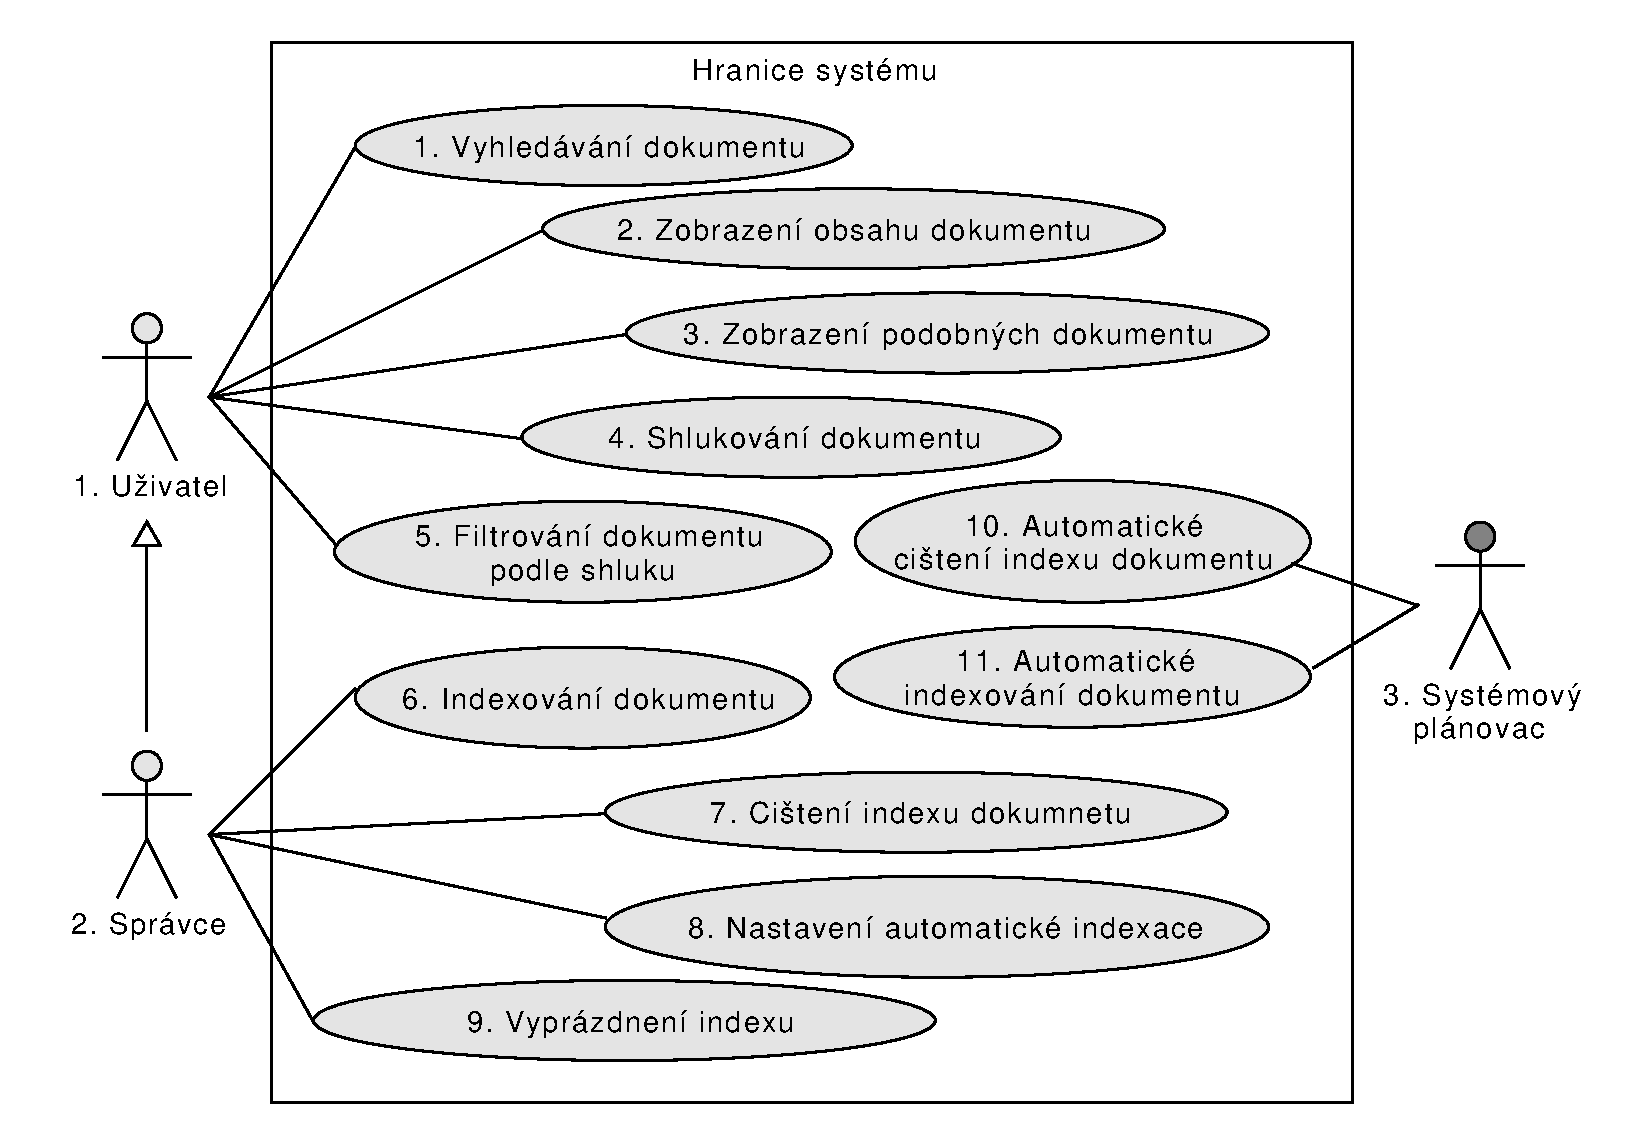
\includegraphics[width=13cm]{UseCases}
\caption{Diagram případů užití}
\label{fig:UseCases}
\end{center}
\end{figure}

\section{Případy užití}

\subsection{Vyhledávání dokumentů}
\begin{itemize}
	\item[Aktéři:] \ref{itm:actor_user} Uživatel
	\item[Scénář:]
	\begin{enumerate}
		\item Uživatel zadá dotaz.
		\item Systém zobrazí výsledky dle dotazu.
	\end{enumerate}
	\item[Výstup:] Dokumenty odpovídající dotazu
\end{itemize}

\subsection{Zobrazení obsahu dokumentů}
\begin{itemize}
	\item[Aktéři:] \ref{itm:actor_user} Uživatel
	\item[Scénář:]
	\begin{enumerate}
		\item Uživatel zvolí zdroj a~zadá dotaz.
		\item Systém zobrazí výsledky dle dotazu.
		\item Uživatel ze zobrazených výsledků vybere požadovaný dokument.
		\item Systém zobrazí obsah dokumentu.
	\end{enumerate}
	\item[Výstup:] Zobrazený obsah dokumentu
\end{itemize}

\subsection{Zobrazení podobných dokumentů}
\begin{itemize}
	\item[Aktéři:] \ref{itm:actor_user} Uživatel
	\item[Scénář:]
	\begin{enumerate}
		\item Uživatel zvolí zdroj a~zadá dotaz.
		\item Systém zobrazí výsledky dle dotazu.
		\item Uživatel ze zobrazených výsledků vybere požadovaný dokument.
		\item Systém zobrazí seznam dalších dokumentů seřazených od nejpodobnějšího k~nejméně podobnému
	\end{enumerate}
	\item[Výstup:] Dokumenty, které jsou podobné zvolenému dokumentu, seřazené od nejpodobnějšího k~nejméně podobnému
\end{itemize}

\subsection{Shlukování dokumentů}
\begin{itemize}
	\item[Aktéři:] \ref{itm:actor_user} Uživatel
	\item[Scénář:]
	\begin{enumerate}
		\item Uživatel zvolí zdroj a~zadá dotaz.
		\item Systém zobrazí jak výsledky dle dotazu, tak nalezené shluky výsledných dokumentů.
	\end{enumerate}
	\item[Výstup:] Seznam shluků výsledných dokumentů
\end{itemize}

\subsection{Filtrování dokumentů podle shluků}
\begin{itemize}
	\item[Aktéři:] \ref{itm:actor_user} Uživatel
	\item[Scénář:]
	\begin{enumerate}
		\item Uživatel zvolí zdroj a~zadá dotaz.
		\item Systém zobrazí výsledky dle dotazu a~nalezené shluky výsledných dokumentů.
		\item Uživatel vybere jeden či více shluků.
		\item Systém zobrazí jen dokumenty patřící do zvolených shluků.
	\end{enumerate}
	\item[Výstup:] Seznam dokumentů v~daných shlucích.
\end{itemize}

\subsection{Indexování dokumentů}
\label{subsec:usecase_index}
\begin{itemize}
	\item[Aktéři:] \ref{itm:actor_admin} Správce
	\item[Scénář:]
	\begin{enumerate}
		\item Správce zvolí jeden či více adresářů.
		\item Systém v~adresářích najde textové soubory a~přidá je do indexu.\label{itm:scenary_index}
	\end{enumerate}
	\item[Výstup:] Zaindexované soubory ze zvolených adresářů připravené pro vyhledávání
\end{itemize}

\subsection{Čištění indexu dokumentů}
\label{subsec:usecase_clean}
\begin{itemize}
	\item[Aktéři:] \ref{itm:actor_admin} Správce
	\item[Scénář:]
	\begin{enumerate}
		\item Správce spustí čištění indexu.
		\item Systém projde dokumenty a~ty, které již neexistují v~souborovém systému, odstraní z~indexu.\label{itm:scenary_clean}
	\end{enumerate}
	\item[Výstup:] Index obsahující pouze dokumenty, které mají svou reprezentaci v~souborovém systému počítače
\end{itemize}

\subsection{Vyprázdnění indexu}
\begin{itemize}
	\item[Aktéři:] \ref{itm:actor_admin} Správce
	\item[Scénář:]
	\begin{enumerate}
		\item Správce spustí vyprázdnění indexu.
		\item Systém odstraní všechny dokumenty z~indexu.
	\end{enumerate}
	\item[Výstup:] Prázdný index
\end{itemize}

\subsection{Nastavení automatické indexace}
\begin{itemize}
	\item[Aktéři:] \ref{itm:actor_admin} Správce
	\item[Scénář:]
	\begin{enumerate}
		\item Správce zvolí interval, adresáře, zda se má indexovat, zda se má čistit index.
		\item Systém ve zvolený čas spouští čištění a~indexaci, viz aktér \ref{itm:actor_scheduler}  Systémový plánovač.
	\end{enumerate}
	\item[Výstup:] Nastavený systémový plánovač
\end{itemize}

\subsection{Automatické indexování dokumentů}
\begin{itemize}
	\item[Aktéři:] \ref{itm:actor_scheduler} Systémový plánovač
	\item[Scénář:]
	\begin{enumerate}
		\item Plánovač nastaví konfiguraci dle nastavení uživatele.
		\item Systém pokračuje v~indexaci od bodu \ref{itm:scenary_index} scénáře \ref{subsec:usecase_index} Indexování dokumentů.
	\end{enumerate}
\end{itemize}

\subsection{Automatické čištění indexu dokumentů}
\begin{itemize}
	\item[Aktéři:] \ref{itm:actor_scheduler} Systémový plánovač
	\item[Scénář:]
	\begin{enumerate}
		\item Plánovač nastaví konfiguraci dle nastavení uživatele.
		\item Systém pokračuje v~indexaci od bodu \ref{itm:scenary_clean} scénáře \ref{subsec:usecase_clean} Čištění indexu dokumentů.
	\end{enumerate}
\end{itemize}

\section{Technologie}
\subsection{Surmon}
Bylo mi navrženo, abych se pokusil implementovat práci pomocí nástroje Surmon. Prostudoval jsem si tedy  dokumentaci aplikace, otestoval si její funkce a~zjistil následující.

Surmon je balík modulů pro platformu OBBB\cite{surmon:guide} --- Open Black Box Builder. Platforma OBBB umožňuje sestavit aplikaci pro zpracování dat pomocí propojování funkčních bloků. Blok je atomický kus algoritmu se vstupy a~výstupy různých datových typů a~s~možností nastavení parametrů pro úpravu jeho chování. Každý blok načte data na svých vstupech, zpracuje je a~výsledná data zapíše na své výstupy. Bloky pak lze propojovat spojnicemi z~výstupu jednoho bloku na vstup jiného --- samozřejmě jen tehdy, jsou-li kompatibilní datové typy vstupů a~výstupů.  Takovouto tvorbou orientovaných grafů bloků a~spojnic lze definovat složité algoritmy. Na sestavování bloků má platforma již vytvořený intuitivní editor v~podobě plátna, na které se bloky přidávají a~kde se propojují. Každý blok má svou reprezentaci v~uživatelském rozhraní, pomocí kterého lze nastavit parametry bloku. Vše je implementováno v~jazyce Java a~postaveno na Platformě NetBeans\cite{netbeans:guide}.

Samotný OBBB obsahuje základní sadu bloků pro řízení toku algoritmu, načítání a~zápis souborů různých formátů, iteraci nad daty a~další funkce. Surmon je pak sada dalších bloků pro operace zpracování textu a~text mining. Pro účely této práce je podstatné zejména to, že Surmon obsahuje bloky pro text mining z~českých textů.

Software tedy umožňuje sestavit algoritmy pomocí hotových celků bez programátorského zásahu. Sestavený alogritmus pak lze uzamknout heslem, vystavit některé vstupy či parametry nastavení jako uživatelské rozhraní a~nabízet vzniklou aplikaci jako hotové řešení.

Platforma umožňuje poměrně snadnou tvorbu nových bloků. Má k~tomu velmi detailně definované a~dokumentované rozhraní. Lze tedy vytvořit bloky pro další dílčí práci s~daty, které následně lze použít stejným způsobem jako bloky vestavěné.

Software Surmon mě velice zaujal, ale pro tuto práci jsem jej nakonec nevyužil. Hlavní problém je v~požadavku klient-server architektury. Zkoumal jsem možnosti rozšířit software pomocí nových bloků tak, aby šel použít i~v~klient-server architektuře, aby například blok začal poslouchat na síťovém portu na příchozí dotazy, nebo aby jen předzpracovával data do indexu, přičemž jiná aplikace by dodávala na základě tohoto indexu výsledky na vyhledávací dotazy. Všechny takové možnosti jsou příliš těžkopádné. Bloky jsou navrhovány jen na přijetí dat, zpracování a~odeslání dat dál v~řetězci. Vstupní  jsou v~programu všechny bloky které nemají vlastní vstupy a bloky se pak postupně zpracovávají v~samostatných vláknech. Při takovém návrhu není snadné zařídit poslouchání na síťovém portu a~odpovídání na požadavky.

Jinými slovy, Surmon je stavěn k~ověřování konceptů různých algoritmů, nebo k~tvorbě jednoúčelového text miningového softwaru jako tzv. standalone aplikace na jednom počítači. Nehodí se na finální řešení k~poskytování služeb přes síťové rozhraní.

Kromě toho, aby mi byl software poskytnut pro implementaci projektu, muselo by být celé textové zpracování implementováno v~Surmonu. Tvůrci Surmonu se totiž snaží bránit jakémukoliv vyvádění implementovaných knihoven ven ze softwaru. Mimo Surmon tedy nelze implementované knihovny využít.

\subsection{Solr}
Protože nástroj Surmon nelze pro můj projekt použít, začal jsem hledat open source software, který by pomohl s~fulltextovým vyhledáváním, byl rozšiřitelný a~zároveň by šel zakomponovat do složitější architektury. Objevil jsem Solr\cite{sorl:wiki}, platformu pro fulltextové vyhledávání vyvíjenou pod licencí Apache License nadací Apache Software Foundation ve spolupráci s~projektem Lucene. 

Solr je napsaný v~jazyce Java, který mu  zajišťuje multiplatformnost, takže může fungovat i~pod systémem Windows, který je zadavatelem preferován.

Solr je vlastně vyhledávací server běžící v~servlet containeru, jako jsou Jetty či Apache Tomcat. Poskytuje REST rozhraní  pro integraci s~jinými aplikacemi v~různých jazycích. Solr v~základní instalaci podporuje hned několik datových formátů pro REST komunikaci, například JSON a~XML. Kromě REST rozhraní jsou k~dispozici již hotové knihovny pro mnoho programovacích jazyků, které ještě více pomohou integrovat Solr s~dalšími aplikacemi. Příkladem je Javová knihovna \emph{SolrJ}, nebo JavaScriptové knihovny \emph{AJAX Solr} nebo \emph{Solr Search}.

Jako fulltextové vyhledávací jádro používá Solr knihovnu Lucene, jejíž funkce zprostředkovává pro samostatné serverové použití. Knihovna Lucene je také napsaná v~jazyce Java, existují však i~její portace do jiných jazyků. Knihovna slouží pro tvorbu a~správu indexu a~následné vyhledávání v~indexu. Na svých stránkách\cite{lucene:wiki} se tvůrci chlubí nízkou náročností na hardware počítače, širokou podporou různých způsobů dotazování, podporou simultálního aktualizace indexu a~vyhledávání, podporou spojování výsledků z~různých indexů a~dalších pokročilých funkcí.

Solr sbírá (indexuje) a~prohledává (dotazuje) index dokumentů. V jedné instanci Solru může být nakonfigurováno více nezávislých indexů --- kolekcí. Dokument je pro Solr jednotka informace. Sestává z~atributů, polí daného datového typu, anglicky fields.  Z~jakých polí se dokument skládá charakterizuje tzv. schéma. To lze nastavit v~konfiguračním souboru \emph{schema.xml}. Všechny dokumenty mají v rámci kolekce stejnou strukturu polí danou schématem. Schéma určuje i~to, jakým způsobem mají být pole interpretována, zpracovávána a~dotazována. Tento proces tvůrci nazývají Field Analysis --- analýza polí. Zde lze například nastavit, jaký tokenizer, stemmer, či filtr se má použít na dané pole. Tyto analyzéry nejsou ničím jiným než Java třídami, které implementují dané rozhraní. Poměrně jednoduše lze tedy vytvořit jakýkoliv vlastní analyzér, který předzpracuje text v~poli.

Solr umožňuje použít k~jednomu poli jeden tokenizer, tj. prvek, který text rozdělí na jednotlivé indexované úseky --- nejčastěji slova. Dále můžeme přiřadit 0--n tzv. char filterů, které očistí text od nepotřebných znaků, jako jsou HTML značky, a~0--n filtrů, které odstraní z~výstupu celá nechtěná slova. Na úryvku XML kódu můžeme pozorovat definice typu pole s~analyzéry zvlášť pro proces indexace a~pro dotazování a~přiřazení tohoto typu pole. V~ukázce si také můžeme všimnout nastavení pole \emph{indexed} a~\emph{stored}. To znamená, že se pole má indexovat a~zároveň se má v~databázi uchovat i~jeho původní plné znění, což je užitečné, jelikož podle indexu se rychle vyhledá daný dokument a~pak se může pole zobrazit ve výsledcích v~plném rozsahu.

V~konfiguraci pole lze povolit i~ukládání vektoru termů. Vektor lze potom využít pro další zpracování textu i~mimo samotný Solr, například při shlukové analýze nebo v~dalších fázích projektu.

Dalšími důležitými nastaveními v~schema.xml jsou: které pole bude unikátní identifikátor dokumentu, ve kterém poli se bude ve výchozím stavu vyhledávat, jaká třída bude vyhodnocovat podobnost dokumentů. Analyzéry mívají ještě další možnosti nastavení.

\begin{verbatim}
<fieldType name="text_general" class="solr.TextField" 
			  positionIncrementGap="100">
 <analyzer type="index">
   <tokenizer class="solr.StandardTokenizerFactory"/>
   <filter class="solr.StopFilterFactory" ignoreCase="true" 
 		     words="stopwords.txt" enablePositionIncrements="true" />
   <filter class="solr.SynonymFilterFactory" 
           synonyms="index_synonyms.txt" 
           ignoreCase="true" expand="false"/>
   <filter class="solr.LowerCaseFilterFactory"/>
 </analyzer>
 <analyzer type="query">
   <tokenizer class="solr.StandardTokenizerFactory"/>
   <filter class="solr.StopFilterFactory" ignoreCase="true" 
           words="stopwords.txt" 
           enablePositionIncrements="true" />
   <filter class="solr.SynonymFilterFactory" 
           synonyms="synonyms.txt"
           ignoreCase="true" expand="true"/>
   <filter class="solr.LowerCaseFilterFactory"/>
 </analyzer>
</fieldType>

<field name="content" type="text_general" 
       indexed="true" stored="true" termVectors="true" />
\end{verbatim}

Zbývá se podívat na to, jak je na tom Solr s~podporou českého jazyka. Podle informací na oficiálních stránkách\cite{sorl:wiki} je Český jazyk nástrojem podporován již od verze 3.5. Lze prý použít standartní tokenizer \emph{StandardTokenizer}, který dělí text na tokeny nejen podle definovaných prázdných znaků, ale má sadu pravidel, která správně nechají v~celku zkratky, slova s~apostrofy a~podobně. K~tomu jsou doporučovány dva běžné filtry: \emph{LowerCaseFilter}, který převede token na malá písmen, a~\emph{StopFilter}, který umožní definovat stop word list, seznam slov, která se mají vynechat z~indexu. Na závěr tvůrci doporučují pro český text použít \emph{CzechStemFilter}. Je to stemmer vycházející z~práce L.~Dolamica a~J.~Savoye, kteří se na Švýcarské University of Neuchatel zabývali stemizačními algoritmy východoevropských jazyků. Stemmer funguje s~tokeny již převedenými do malých písmen a~umí pracovat s~diakritikou. Funguje na principu postupného odebírání koncovek a~některých předpon slov.

Výsledky analýzy nástroje Solr lze tedy shrnout takto: Solr se zdá být vhodným kandidátem pro nasazení v~projektu. Neklade meze integraci s~jinými aplikacemi a~do jisté míry podporuje český jazyk. Nepochybně ale bude nutné otestovat kvalitu zpracování českých textů a~popřípadě nástroj rozšířit o~nové knihovny pro tento účel.

\subsection{Jetty}
Solr jako Java EE aplikace potřebuje servlet container ke svému běhu --- Jetty. Jetty\cite{jetty:doc} je open source javový web server a~java servlet container, vyvíjený společností Eclipse Foundation. Pro projekt jsem zvažoval i~použití Apache Tomcat\cite{tomcat:doc}, se kterým už mám zkušenost z~předchozích projektů, ale narazil jsem na několik chyb a~nekompatibilit se Solrem. Zůstal jsem tedy nakonec u~Jetty, se kterým se Solr oficiálně distribuuje a~který oficiálně podporuje.

\subsection{Carrot2}
Jedním z~požadavků na projekt je shlukování výsledků vyhledávání. Zjistil jsem, že existuje javový open source shlukovací engine Carrot2\cite{carrot2:manual}, který má podporu v~jádře Solru. Engine je určený pro shlukování spíše menších kolekcí dat a~hodí se tedy právě pro shlukování výsledků vyhledávání.

Carrot2 se distribuuje se třemi implementovanými algoritmy pro shlukování. Obsahuje algoritmus Bisekční K-means, který počítá vzdálenosti vektorů dokumentů nebo vektoru reprezentantů shluků a~vždy do shluku spojí dva nejbližší sousedy až do požadovaného počtu shluků. Dále obsahuje algoritmus Lingo, který vytvořili S.~Osiński, J.~Stefanowski a~D.~Weiss, založený na algebraických transformacích matic termů a~extrakci častých frází použitím sufixových polí. Posledním obsaženým algoritmem je STC, suffix tree clustering, který sestaví termy do sufixového stromu, aby nalezl prvotní zástupce shluků dokumentů.

Carrot2 obsahuje i~J2EE webovou aplikaci s~hotovým vyhledávacím rozhraním. Tato aplikace má možnost nakonfigurovat i~několik informačních zdrojů, ve kterých se bude vyhledávat. V~základu je několik zdrojů implementováno. Můžeme aplikaci napojit například na Wikipedii, Google, Bing i~Solr. Aplikace již podporuje zvýraznění hledaných slov ve výsledcích, zobrazení shluků i~filtrování dokumentů podle zvoleného shluku. Funguje tím způsobem, že dotaz přepošle na zdrojovou službu a~nad výsledky, které jí služba vrátí provede shlukovou analýzu. Následně pak zobrazí výsledky vyhledávání i~nalezené shluky. Shluky navíc umí zobrazit i~interaktivně v~grafické formě.

Carrot2 lze tedy k~Solru připojit dvěma způsoby. Jednou možností je nasadit Carrot2 jako samostatnou webovou aplikaci, která bude zprostředkovávat vyhledávací dotazy na Solr server a~výsledky vyhledávání před vrácením ještě podrobí shlukové analýze. V~tomto případě by ale musel Carrot2 být zároveň i~frontendem systému a~tak využiji druhé možnosti připojení: Carrot2 bude do Solru nainstalován a~nakonfigurován jako rozšiřující knihovna pro shlukování výsledků, která bude obohacovat výsledky vyhledávání o~výsledky shlukové analýzy. Tím se zachová možnost výběru frontendu.